\documentclass[journal]{vgtc}                % final (journal style)
%\documentclass[review,journal]{vgtc}         % review (journal style)
%\documentclass[widereview]{vgtc}             % wide-spaced review
%\documentclass[preprint,journal]{vgtc}       % preprint (journal style)

%% Uncomment one of the lines above depending on where your paper is
%% in the conference process. ``review'' and ``widereview'' are for review
%% submission, ``preprint'' is for pre-publication, and the final version
%% doesn't use a specific qualifier.

%% Please use one of the ``review'' options in combination with the
%% assigned online id (see below) ONLY if your paper uses a double blind
%% review process. Some conferences, like IEEE Vis and InfoVis, have NOT
%% in the past.

%% Please note that the use of figures other than the optional teaser is not permitted on the first page
%% of the journal version.  Figures should begin on the second page and be
%% in CMYK or Grey scale format, otherwise, colour shifting may occur
%% during the printing process.  Papers submitted with figures other than the optional teaser on the
%% first page will be refused. Also, the teaser figure should only have the
%% width of the abstract as the template enforces it.

%% These few lines make a distinction between latex and pdflatex calls and they
%% bring in essential packages for graphics and font handling.
%% Note that due to the \DeclareGraphicsExtensions{} call it is no longer necessary
%% to provide the the path and extension of a graphics file:
%% 
\includegraphics{diamondrule} is completely sufficient.
%%
\ifpdf%                                % if we use pdflatex
  \pdfoutput=1\relax                   % create PDFs from pdfLaTeX
  \pdfcompresslevel=9                  % PDF Compression
  \pdfoptionpdfminorversion=7          % create PDF 1.7
  \ExecuteOptions{pdftex}
  \usepackage{graphicx}                % allow us to embed graphics files
  \DeclareGraphicsExtensions{.pdf,.png,.jpg,.jpeg} % for pdflatex we expect .pdf, .png, or .jpg files
\else%                                 % else we use pure latex
  \ExecuteOptions{dvips}
  \usepackage{graphicx}                % allow us to embed graphics files
  \DeclareGraphicsExtensions{.eps}     % for pure latex we expect eps files
\fi%

%% it is recomended to use ``\autoref{sec:bla}'' instead of ``Fig.~\ref{sec:bla}''
\graphicspath{{figures/}{pictures/}{images/}{./}} % where to search for the images

\usepackage{microtype}                 % use micro-typography (slightly more compact, better to read)
\PassOptionsToPackage{warn}{textcomp}  % to address font issues with \textrightarrow
\usepackage{textcomp}                  % use better special symbols
\usepackage{mathptmx}                  % use matching math font
\usepackage{times}                     % we use Times as the main font
\renewcommand*\ttdefault{txtt}         % a nicer typewriter font
\usepackage{cite}                      % needed to automatically sort the references
\usepackage{tabu}                      % only used for the table example
\usepackage{booktabs}                  % only used for the table example
%% We encourage the use of mathptmx for consistent usage of times font
%% throughout the proceedings. However, if you encounter conflicts
%% with other math-related packages, you may want to disable it.

%% In preprint mode you may define your own headline.
%\preprinttext{To appear in IEEE Transactions on Visualization and Computer Graphics.}

%% If you are submitting a paper to a conference for review with a double
%% blind reviewing process, please replace the value ``0'' below with your
%% OnlineID. Otherwise, you may safely leave it at ``0''.
\onlineid{0}

%% declare the category of your paper, only shown in review mode
\vgtccategory{Research}
%% please declare the paper type of your paper to help reviewers, only shown in review mode
%% choices:
%% * algorithm/technique
%% * application/design study
%% * evaluation
%% * system
%% * theory/model
\vgtcpapertype{please specify}

%% Paper title.
\title{FencingVis}

%% This is how authors are specified in the journal style

%% indicate IEEE Member or Student Member in form indicated below
\author{Roy G. Biv, Ed Grimley, \textit{Member, IEEE}, and Martha Stewart}
\authorfooter{
%% insert punctuation at end of each item
\item
 Roy G. Biv is with Starbucks Research. E-mail: roy.g.biv@aol.com.
\item
 Ed Grimley is with Grimley Widgets, Inc.. E-mail: ed.grimley@aol.com.
\item
 Martha Stewart is with Martha Stewart Enterprises at Microsoft
 Research. E-mail: martha.stewart@marthastewart.com.
}

%other entries to be set up for journal
\shortauthortitle{Biv \MakeLowercase{\textit{et al.}}: Global Illumination for Fun and Profit}
%\shortauthortitle{Firstauthor \MakeLowercase{\textit{et al.}}: Paper Title}

%% Abstract section.
\abstract{Duis autem vel eum iriure dolor in hendrerit in vulputate
velit esse molestie consequat, vel illum dolore eu feugiat nulla
facilisis at vero eros et accumsan et iusto odio dignissim qui blandit
praesent luptatum zzril delenit augue duis dolore te feugait nulla
facilisi. Lorem ipsum dolor sit amet, consectetuer adipiscing elit,
sed diam nonummy nibh euismod tincidunt ut laoreet dolore magna
aliquam erat volutpat. Ut wisi enim ad minim veniam, quis nostrud exerci tation ullamcorper
suscipit lobortis nisl ut aliquip ex ea commodo consequat. Duis autem
vel eum iriure dolor in hendrerit in vulputate velit esse molestie
consequat, vel illum dolore eu feugiat nulla facilisis at vero eros et
accumsan et iusto odio dignissim qui blandit praesent luptatum zzril
delenit augue duis dolore te feugait nulla facilisi.%
} % end of abstract

%% Keywords that describe your work. Will show as 'Index Terms' in journal
%% please capitalize first letter and insert punctuation after last keyword
\keywords{Radiosity, global illumination, constant time}

%% ACM Computing Classification System (CCS). 
%% See <http://www.acm.org/class/1998/> for details.
%% The ``\CCScat'' command takes four arguments.

\CCScatlist{ % not used in journal version
 \CCScat{K.6.1}{Management of Computing and Information Systems}%
{Project and People Management}{Life Cycle};
 \CCScat{K.7.m}{The Computing Profession}{Miscellaneous}{Ethics}
}

%% Uncomment below to include a teaser figure.
\teaser{
  \centering
  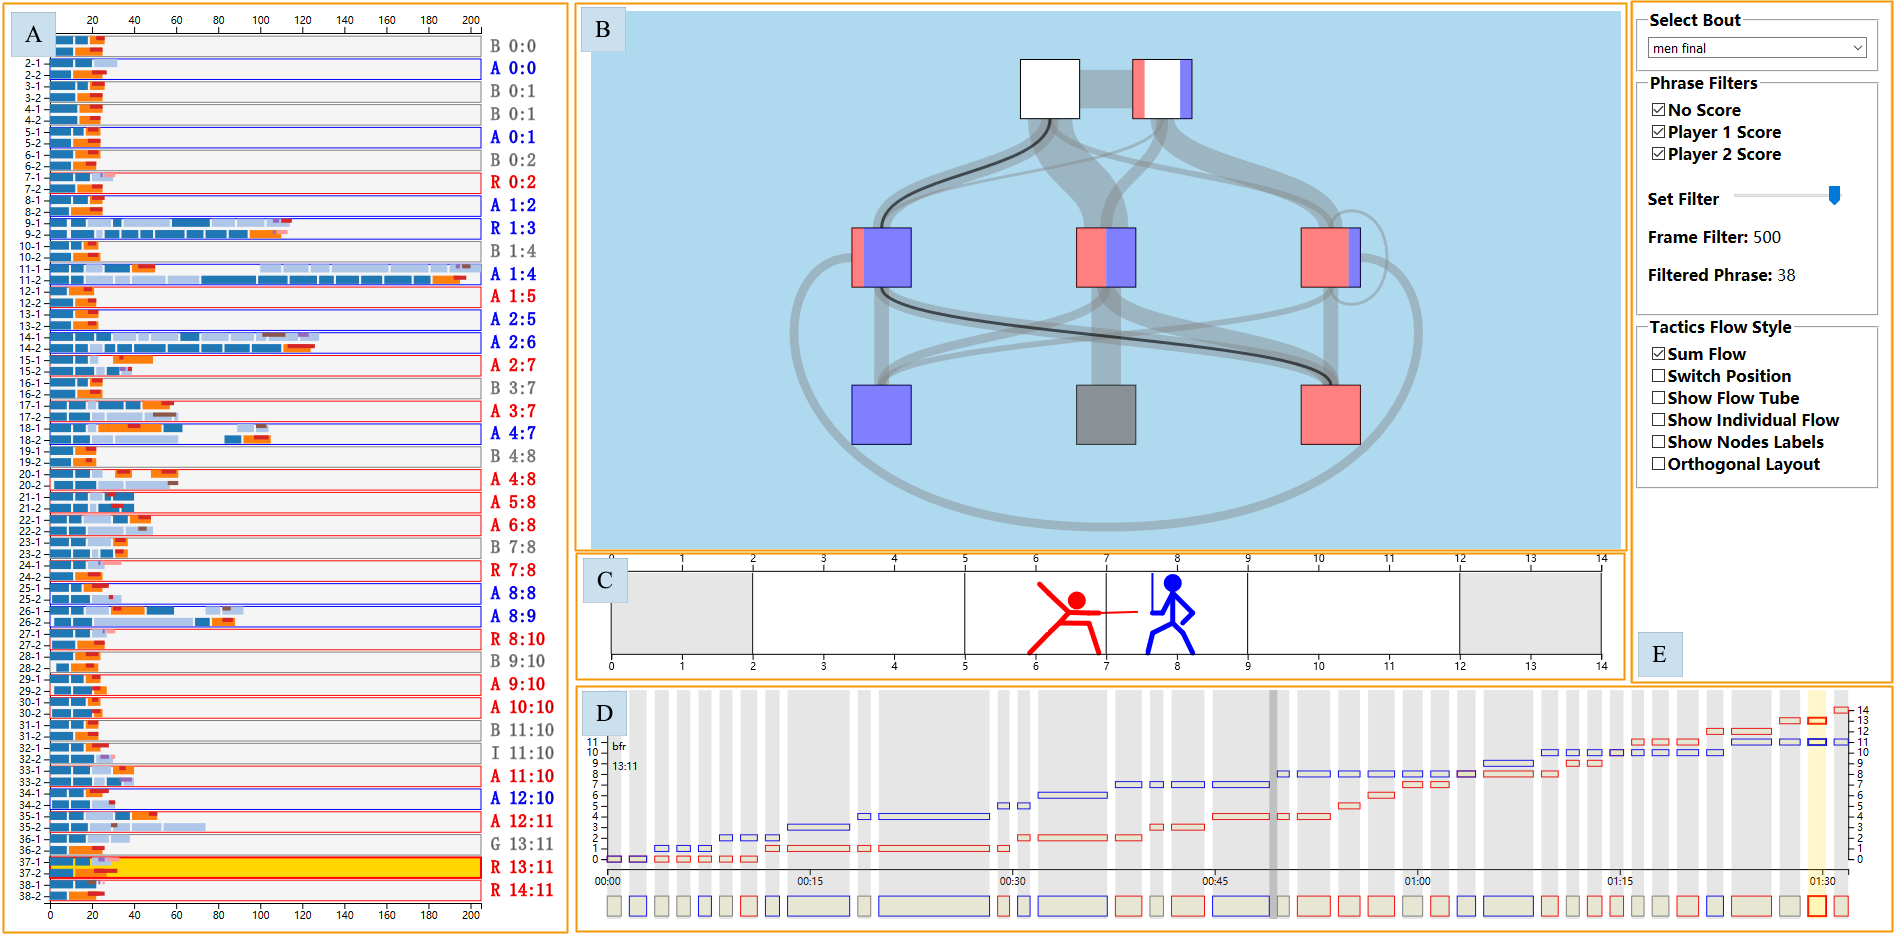
\includegraphics[width=\linewidth]{main}
  \caption{The main picture of FencingVis. A) Motion View. B) Tactic Flowchart View. C) Phrase View. D) Bout View. E Control Pannel}
	\label{fig:teaser}
}

%% Uncomment below to disable the manuscript note
%\renewcommand{\manuscriptnotetxt}{}

%% Copyright space is enabled by default as required by guidelines.
%% It is disabled by the 'review' option or via the following command:
% \nocopyrightspace

\vgtcinsertpkg

%%%%%%%%%%%%%%%%%%%%%%%%%%%%%%%%%%%%%%%%%%%%%%%%%%%%%%%%%%%%%%%%
%%%%%%%%%%%%%%%%%%%%%% START OF THE PAPER %%%%%%%%%%%%%%%%%%%%%%
%%%%%%%%%%%%%%%%%%%%%%%%%%%%%%%%%%%%%%%%%%%%%%%%%%%%%%%%%%%%%%%%%

\begin{document}

%% The ``\maketitle'' command must be the first command after the
%% ``\begin{document}'' command. It prepares and prints the title block.

%% the only exception to this rule is the \firstsection command
\firstsection{Introduction}

\maketitle

%% \section{Introduction} %for journal use above \firstsection{..} instead

The development of information technology makes the data recorded in sports more and more comprehensive and detailed, which leads to the research on the visualization and visual analysis of sports data.
Sports data visualization and visual analysis work for a wide range of groups, mainly can be divided into four categories.
Methods for general sports enthusiasts focus on the display of big data, so that sports enthusiasts can more intuitive and quick access to their own information of interest, as well as provide some simple analysis and prediction results.
Methods for professional teams of athletes and coaches focus on exploring the technical and tactical characteristics behind the data, thus providing guidance for training and tactical use.
There are also efforts aimed at relevant sports associations and operators, often requiring analysis of larger-scale data to provide strategic guidance for their future operations.
According to the design of sports researchers need to combine the knowledge of biomechanics, psychology and other fields, to assist researchers to complete their relevant experimental analysis.
Previous data analysis and visualization efforts for fencing were relatively small.
Although the sport has a long history and has been playing a role in major competition systems such as the Olympic games, it is more difficult to understand than other sports and therefore attracts fewer groups.
In addition, fencing competition time is short, fast pace, many times even professional fencer and referee will produce different understanding.
So for this sport, the display of the game not only for ordinary enthusiasts, professionals also exist in this aspect of the demand, this has been unified in the analysis of the demand.
In addition, fencing competition data do not have the natural structure, need to extract its structural data, and this work is a basic work for the display and analysis of the game.
In view of the above requirements, we design a visual analysis system.
First, we extract the original data of fencing competition in a structured way.
After that, we show from different dimensions of time, space, statistics and so on, and on this basis to provide professionals for technical and tactical analysis of interactive exploration.
Our main contributions:
\begin{enumerate}
	\item We have structured definitions of fencing competition data and provide conversion from raw data to structured data.
	\item We design a variety of different views to present the transformed structured data in all directions and angles.
	\item We provide a series of interactive methods and view correlation to help professionals explore and find technical and tactical problems in the game, to better develop training plans and arrange the game strategy.
	\item We conducted user analysis of fencing athletes and coaches, as well as case studies of international competitions, which proved that our system could help them get new intuiation.
\end{enumerate}

\section{Related Work}
Our work is mainly related to the analysis of fencing data and sports data visualization and visual analysis, so we first introduce the related work in these two areas.

\subsection{Analysis and Visualization for Fencing}
The existing data analysis for fencing mainly focus on biomechanics category, through the analysis of competition data to send the difference between excellent fencers and beginners, so as to clear the focus of training\cite{chen2017biomechanics}. But these works are completely from the technical level, did not consider the improvement of tactical ability. 
Previous studies have also used statistical methods for time series analysis of fencing competition data\cite{tarrago2016complementary}. These studies use the existing empirical model to collect data, and the game process is summarized as a combination of several known patterns\cite{tarrago2015analisis}. We use this description of the game for reference, but at the recording level we choose to record the most primitive data, such as the movements of the steps and the movements of the hands. This can reduce the cost and information loss caused by introducing domain knowledge into the data acquisition process. We put the data abstraction work in the subsequent analysis process, doing so will bring a variety of benefits. First of all, the behavior pattern of different sword species is different, but at the most basic level is the hands and feet of all kinds of actions, we can use a unified format to record data, and in the logic of processing to distinguish it. In addition, if these empirical models change in the future, we can modify the logic of the system without having to recapture the data.

\subsection{Sports Visualization and visual analytics}
The visualization and visual analysis of sports data has developed vigorously in the past two decades, but there are still many opportunities and challenges.
Basole et. al. summarized two major difficulties in visualizing sports data\cite{basole2016sports}.
In addition to the complexity of the data, the main dilemma facing sports data visualization is the wide range of users, and different users' needs vary greatly.
Previous work has often targeted the needs of a particular class of users.
Some for general sports enthusiasts, some for professional athletes and coaches, some for related sports institutions and operators, some for psychological and physiological related researchers.

From the analysis of the data range, sports data visualization work can also be classified into four categories.
There is some work for a full tournament or league season, showing the points and rankings of each team during the season\cite{perin2016using}, or providing support for game forecasting\cite{vuillemot2016sports}.
The other is for a game, showing the dynamics of the situation in the game and the information on both sides of the game.
Some of the work is aimed at multi-player games, such as football, basketball, they focus on the spatial information of athletes, and analyze the space reflects the tactical layout of the impact on the game.\cite{sacha2014feature,perin2013soccerstories}.
Others focus on showing and analyzing the use of tactics or ability characteristics for individual athletes.\cite{polk2014tennivis,wu2018ittvis}
There are also games that compare multiple games. 
The last category deals with certain scenarios for a particular athlete or game.

Our work is for a single-player game, and two previous jobs are similar to our scenario.
TenniVis\cite{polk2014tennivis} uses the score and serve data to analyze amateur tennis matches.
iTTVis\cite{wu2018ittvis} uses more specialized data, such as placement and batting techniques, to analyze table tennis data more professionally.
Their method does not apply to fencing data because fencing has different characteristics compared to tennis and table tennis.
First of all, tennis and table tennis each round will end with one score, and fencing is not the case, some rounds can be both sides do not score, and some rounds both sides score (epee), which requires different visual design.
In addition, priority rules in fencing competition is very important, and the judgment of this information needs some professional knowledge.
If you can't judge the ownership of the priority, you can't understand the fencing score.
Therefore, the demonstration of priority is very important to the understanding of fencing competition.
We summarize the characteristics of fencing that need to be considered in visual design:
\begin{itemize}
	\item Fencing is not as easy to understand as tennis, table tennis, etc.
	It is often difficult for inexperienced users to read games directly.
	Therefore, the visual design needs to be able to help users better understand the game.
	\item In most sports competitions, the current field information is clear, but the most important priority information in fencing is not clear.
	People with different experiences may have different understandings, which involves the visualization of uncertainty.
	\item Most sports are bound to end each round with one side scoring, but fencing is not the case.
	Both sides may not score points or score points at the same time in a phrase, which also needs special design to reflect.
	\item The use of tactics is more important in fencing than in sports that place more emphasis on adaptability.
	And fencing tactics are often planned in advance before each phrase, so it is more valuable to show the impact of this strategy on the game.
\end{itemize}
In addition, fencing is divided into epee, foil, and sabre.
The three have both similarities and their own characteristics.
Therefore, showing the differences between the three is also one of the design goals of visualization system.


\section{Background and System Overview}
We will introduce the background knowledge of fencing, as long as the data we used and the analysis target. We will also give the main picture of our system.
\subsection{Background}
Fencing is one of the representative events of the Olympic games, which developed from the fencing used for military combat and duel in the cold weapon era.
Fencing consists of epee, foil, and sabre, all of which score by hitting the opponent's active part.
The basic techniques of fencing are divided into offensive techniques and defensive techniques.
Attack techniques include attack, riposte, feint, lunge, beat attack, disengage, compound attack, continuation/renewal of attack, and flick.
Defense techniques include parry, circle parry, counter attack, point-in-line.
These techniques are implemented by a limited combination of hand and foot movements.
Fencing competition is divided into individual and group competition, there are two stages of group competition and group competition.
The individual's first 15 points out of the group game to win ( heavy sword or foil after playing full game time score more victory ).
After one player has scored eight points in the sabre match, the two sides will take a minute off.


	
\subsection{Data Description}
Because of the fast pace of fencing, it is difficult to record the details of the match in real time.
And in order to avoid interfering with the competitors, it is not convenient to install the sensor device.
The existing analysis of fencing competition is achieved through the video of the game, we also extract data from the game video data.
Because of the accuracy of the general game video is 30 frames per second, we record data frame by frame, time accuracy is 1/30 seconds. For each frame of data, we record the listing attributes:
\begin{enumerate}
	\item Footwork of both sides: Record the start and end of forward, backward, and lunge.
	\item Blade work of both sides: Record the start and end of attack, antiattack, parry, and riposte.
	\item Position in the strip.
	\item Result: The referee's decision on the current phrase.
	\item Score: Record which player scored or none.
	\item Sequence: sequence of the current phrase.	
\end{enumerate} 
In the process of data marking, continuous footwork is not easy to effectively segmentation.
After consulting the domain experts, we use the start time of the next action as the segmentation point of the two actions.
Such as continuous forward we use each front foot lift as a segmentation point, continuous back we use each rear foot lift as a segmentation point.

\subsection{Requirement Analysis}
Through ongoing exchanges and discussions with field experts, we have initially identified system needs:
\begin{itemize}
	\item (R1) Show how the game changes over time
	\begin{itemize}
		\item (R1a) Show changes in scores
		\item (R1b) Shows how long each turn lasts
	\end{itemize}
	\item (R2) Show a detailed comparison of the actions of each phrase
	\item (R3) Show how the tactics of both sides were used throughout the game
	\item (R4) Exploratory pattern discovery and result communication
\end{itemize}
\subsection{System Overview}
Our system consists of five forms, as shown in \autoref{fig:teaser}
\section{FencingVis}
\subsection{Bout View}
Almost all game data naturally have time attributes, and both tactical and technical analysis need to consider the impact of time.
The influence of time is reflected in two aspects.
First of all, different stages of the game, the athlete's psychological and physical changes, which has an important impact on the results of the game.
In addition, the use of tactics is also time - dependent.
The fencer will choose the next tactics based on the tactics he or she and his or her opponent have used over a period of time.
Such as the choice of repetition or conversion, need to be determined according to the characteristics of the previous game and the opponent.
Therefore, it is very important for analysts to show the changes of competition over time.

The bout view mainly shows three elements, time, score change and phrase duration.
We use a tailored step chart to show the variation of scores according to time.
X - axis mapping game time, y - axis mapping score.
Red and blue rectangles represent scores for both sides, respectively.
The two rectangles naturally overlap in purple when they are equal-scored.
To visually compare the duration of each turn, we add a horizontal rectangle below the x - axis to show each phrase.
The color of the rectangle indicates the player who scores in this phrase, and the gray indicates that neither side scores.
The upper and lower views correspond to each other, helping the user visually observe the relationship between the three attributes.
Since the break between the first and second half often has a greater impact on the course of the game, we use a vertical line to emphasize this split moment.
When making a selection of the phrase, we use a gray background to reflect the selection of the phrase.

Description: The game time in our view does not exactly correspond to the natural time.
Since the time in the fencing phrases accounts for a small proportion of the actual time, the view becomes very sparse if mapped directly.
So we map the time in the phrases equally, and map the time between two adjacent rounds all to one second interval.

\subsection{Motion View}

\begin{figure*}[tb]
	\centering
	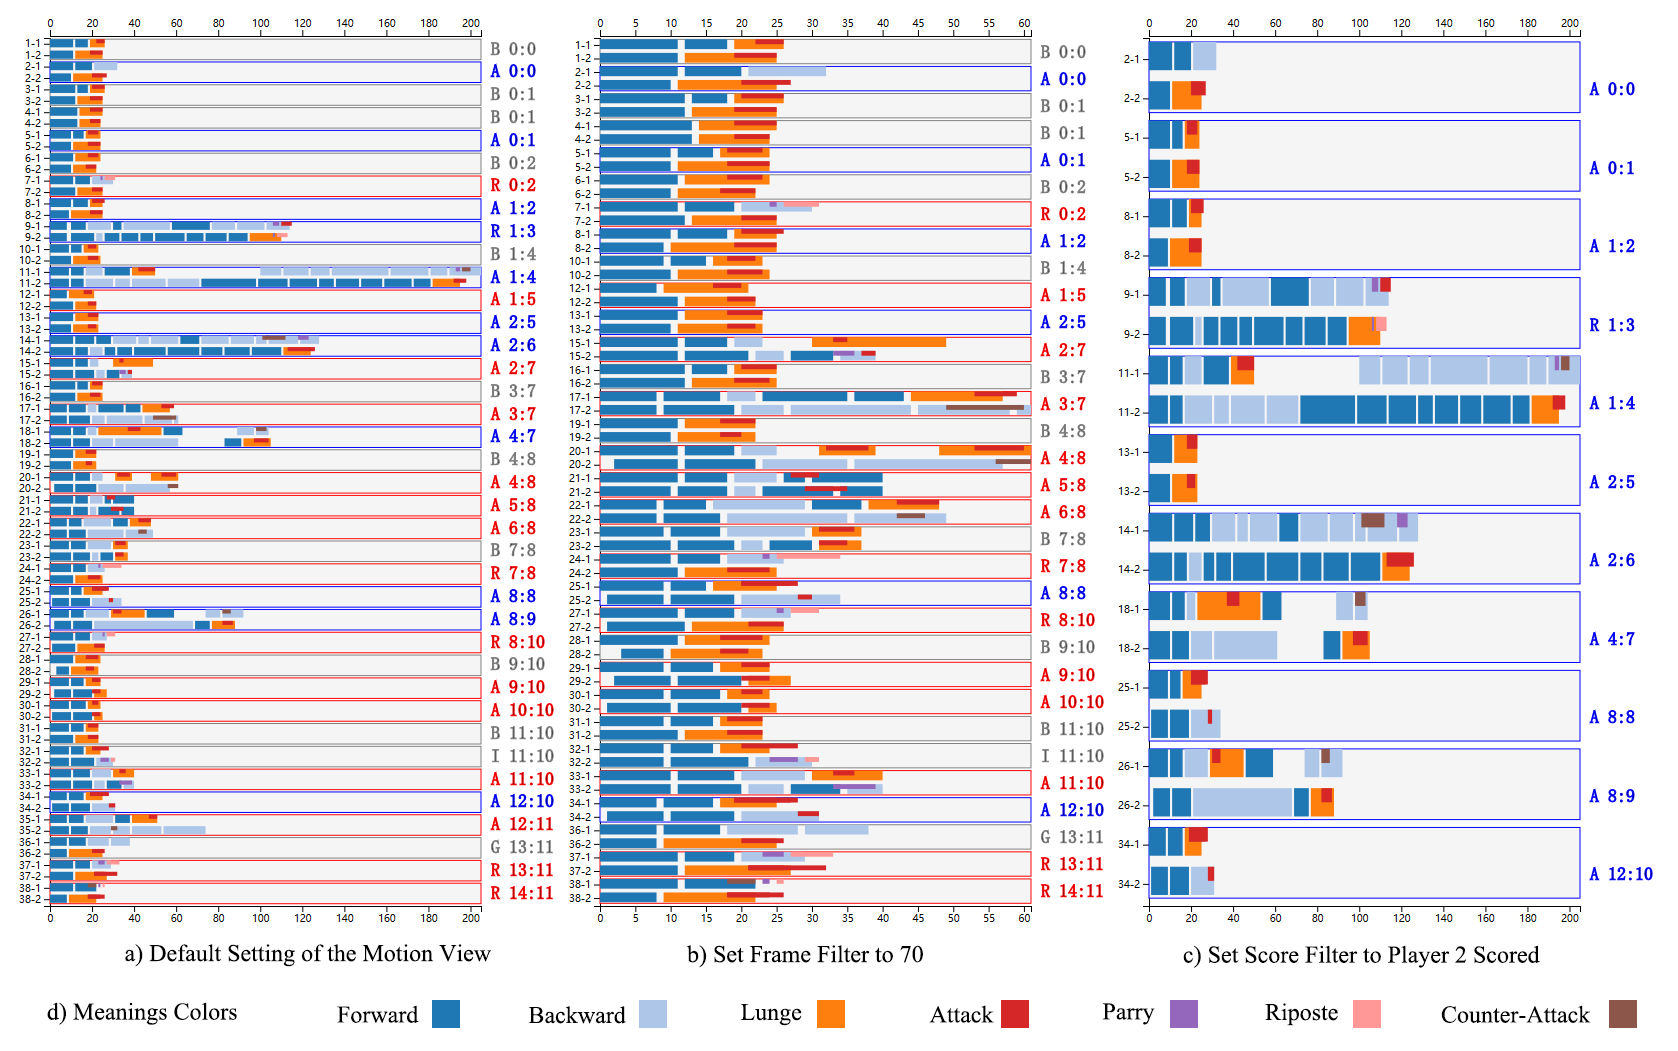
\includegraphics[width=\linewidth]{motionview}
	\caption{Motion View}
	\label{fig:motionview}
\end{figure*}

\subsection{Tactic Flow View}
\subsection{Animation Replay}
\begin{figure}[tb]
	\centering
	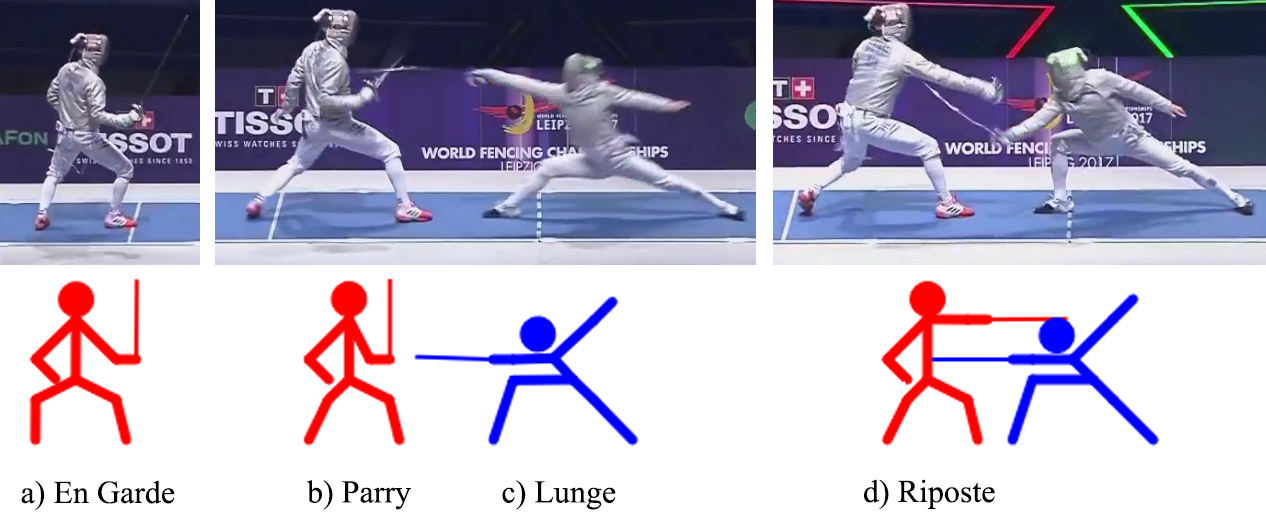
\includegraphics[width=\columnwidth]{glyph}
	\caption{A visualization of the data from \autoref{tab:vis_papers}. The image is from \cite{Isenberg:2017:VMC} and is in the public domain.}
	\label{fig:sample}
\end{figure}
\subsection{Interaction}
\subsection{Cross-View Analysis}

\section{Case Study}
\subsection{Men's Sabre Individual Golden Match of 2017 World Fencing Championships}

\subsection{Comparison of Three Bouts}

\begin{figure*}[tb]
	\centering
	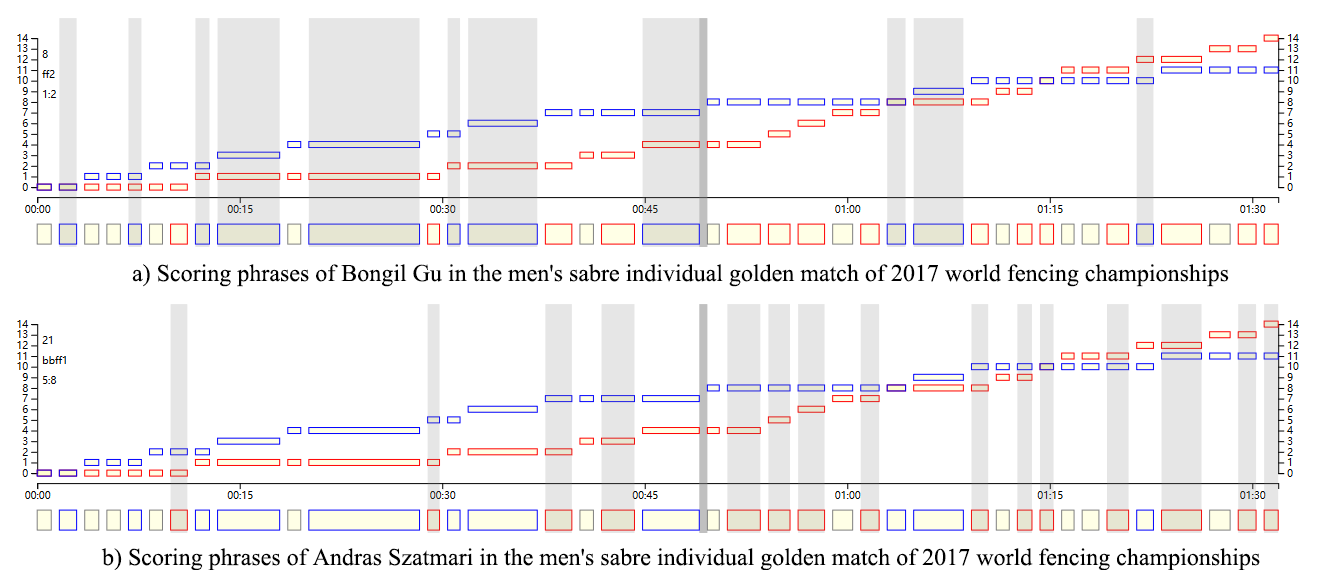
\includegraphics[width=\linewidth]{ScorePhrases}
	\caption{Bout View}
	\label{fig:boutview}
\end{figure*}
\begin{figure*}[tb]
	\centering
	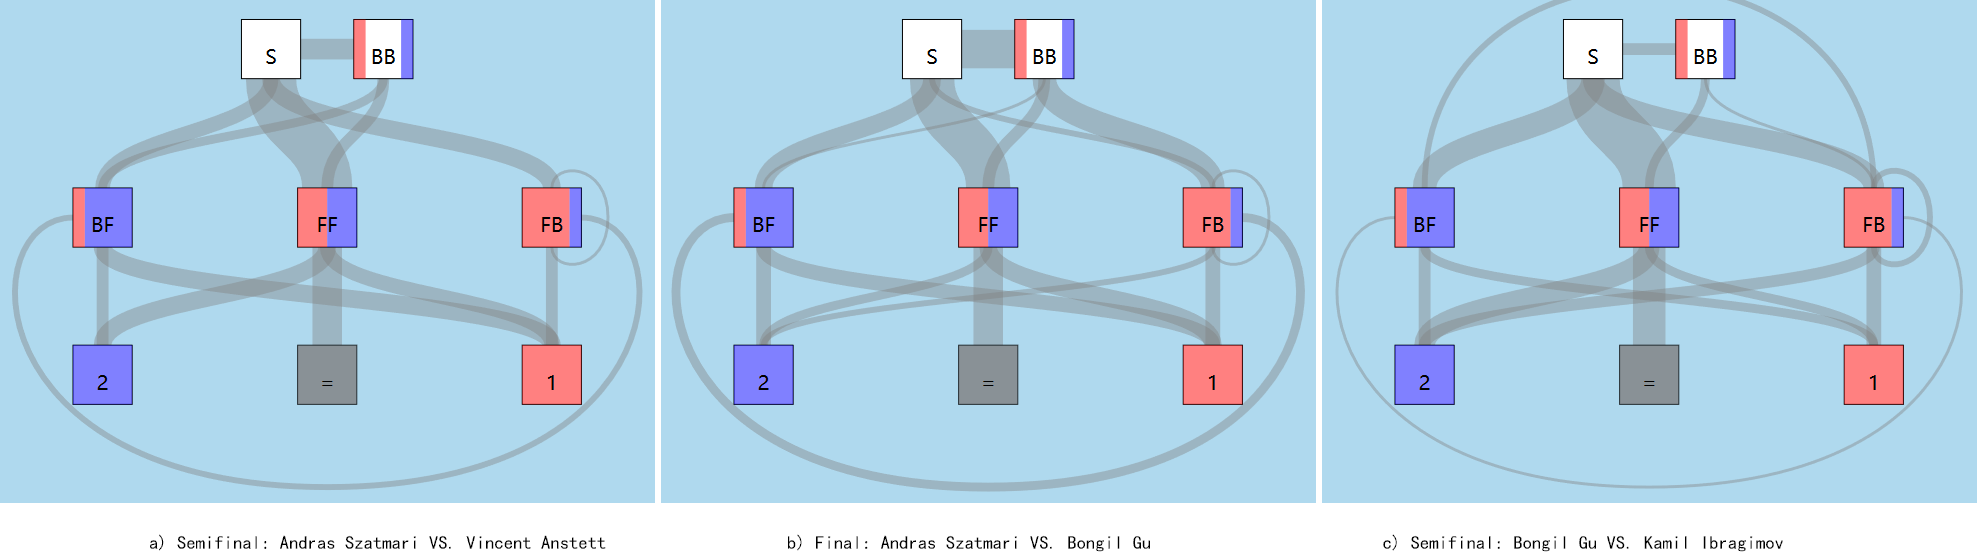
\includegraphics[width=\linewidth]{threeBout}
	\caption{A visualization of the data from \autoref{tab:vis_papers}. The image is from \cite{Isenberg:2017:VMC} and is in the public domain.}
	\label{fig:sample}
\end{figure*}

\section{Conclusion}





%% if specified like this the section will be committed in review mode
\acknowledgments{
The authors wish to thank A, B, C. This work was supported in part by
a grant from XYZ.}

%\bibliographystyle{abbrv}
\bibliographystyle{abbrv-doi}
%\bibliographystyle{abbrv-doi-narrow}
%\bibliographystyle{abbrv-doi-hyperref}
%\bibliographystyle{abbrv-doi-hyperref-narrow}

\bibliography{FencingVis}
\end{document}

